
\documentclass[conference]{IEEEtran}

% Required Packages
\usepackage{stmaryrd}
\usepackage{amsfonts}

% Additional Packages
\usepackage{amsmath}
\usepackage{graphicx}
\usepackage{url}
\usepackage{epstopdf}
\usepackage{array}
\usepackage{multirow}
\usepackage{rotating}

% correct bad hyphenation here
%\hyphenation{op-tical net-works semi-conduc-tor IEEEtran}

\IEEEoverridecommandlockouts
\textwidth 178mm
\textheight 239mm
\oddsidemargin -7mm
\evensidemargin -7mm
\topmargin -6mm
\columnsep 5mm

\begin{document}

\title{\ \\ \LARGE\bf Issues on Sampling Negative Examples for Predicting Prokaryotic Promoters\thanks{
Eduardo G. Gusm\~{a}o is with the RWTH Aachen University Medical School, Institute for Biomedical Engineering, IZKF Aachen Computational Biology Research Group, Aachen, Germany (email: eduardo.gusmao@rwth-aachen.de).
Marcilio C. P. de Souto is with the Univ. Orl\'{e}ans, INSA Centre Val de Loire, LIFO EA 4022, FR-45067, Orl\'{e}ans, France (email: marcilio.desouto@univ-orleans.fr).
}
\thanks{Marcilio C. P. de Souto is also with Univ. Federal de Pernambuco, Centro de Infom\'{a}tica (CIn), Recife, Brazil. This work was partially supported by the Interdisciplinary Center for Clinical Research (IZKF Aachen), RWTH Aachen University Medical School, Aachen, Germany; and Brazilian research agency FACEPE.}
}

\author{Eduardo G. Gusm\~{a}o and Marcilio C. P. de Souto}

%\specialpapernotice{(Invited Paper)}

\maketitle

\begin{abstract}
Supervised learning methods have been successfully used to build classifiers for the identification of promoter regions. The classifier is often built from a dataset that has examples of promoter (positive) and non-promoter (negative) regions. Thus, a careful selection of the data used for constructing and evaluating a promoter finding algorithm is a very important issue. In this context, experimentally known promoter regions can be safely assumed to be positive training instances. In contrast, since definite knowledge whether a given region represents a non-promoter is not generally available, negative instances are not straightforward to be obtained. To make the problem more complex, for the case of promoter, there is not a unique definition of what a negative instance is. As a consequence, depending on which definition of non-promoter region one assumed to build the data, such a choice could affect significantly the performance of the classifier and/or yield a biased estimate of the performance. We present an empirical study of the effect of this kind of problem for promoter prediction in {\it E. coli}. As far as we are concerned, up to now, there is no such a kind of study for the context of prokaryotic promoter prediction.
\end{abstract}

\section{Introduction}
\label{sec:intro}

The problem with negative sampling is common in many areas of bioinformatics such as prediction of mRNAs that are target of miRNAs, regulatory networks, protein-protein interactions, non-coding RNA finding, among others \cite{bandyopadhyay2009,cerulo2010,park2011,wang2006}. For instance, in the studies of miRNA target the majority of the methods suffer from high rates of false positives or false negatives. This happens mostly because systematic identification of mRNAs not proven to be target of miRNAs is still not addressed properly. Thus, current machine learning methods have to rely on artificially generated negative examples for training \cite{bandyopadhyay2009}. Likewise, regulatory networks modeling and protein-protein interactions share the problem that definite knowledge is typically not available that a given pair of genes, proteins or other products under study do not interact \cite{cerulo2010,park2011}. This problem  also arises in the context of prokaryotic promoter prediction.  In fact, in this paper, we present an empirical study of the effect of this problem -- negative sampling -- in the context of prokaryotic promoter prediction.

Promoter prediction in prokaryotes is often modeled as a binary classification task: the algorithm should generate a classifier able to discriminate between promoter (positive) and non-promoter (negative) regions. These samples are frequently nucleotide sequences (primary sequence) or features extracted from them. 

There is a great deal of work in this context of promoter prediction in prokaryotes as a classification problem. In early studies, Norton~\cite{norton1994} made interesting observations about the methodological issues concerning sequence extraction from consensus genomes. He developed a probabilistic method to predict promoters by evaluating uncertainty in the training data. Helmann~\cite{helmann1995} analyzed 236 {\it B. subtilis} promoters recognized by ${\sigma }^{{A}}$-RNA polymerase and demonstrated interesting characteristics concerning conserved positions and dinucleotide frequency patterns. 

More recently, Dhar \cite{dhar2010} reviewed the use of features such as curvature, bendability and stability to try to build more accurate classifiers. Wu et al~\cite{wu2011} improved the prediction accuracy with a method that considered the correlations between nucleotides at the construction of position weight matrices representing the promoters. In another interesting work, the authors performed neural networks simulations based both on the primary sequences (nucleotide sequences) and other features expressing sequences in terms of their free energy~~\cite{avila2011}.

However, independently of the algorithm used to generate the classifiers or the type of attributes used to represent the instances in the dataset (primary sequence and/or its features), one methodological issue that researchers have to account for is the construction/choice of the negative instances. This is the main of concern of this paper. For example, currently there are many experimentally known promoter regions that can safely be assumed to be positive training instances. In contrast, it is experimentally complex to prove that a sequence does not contain a promoter. As a consequence, negative examples have been obtained in alternative ways, each one of them leading to different ``definitions'' for what a negative example is. 

Thus, depending on which definition (or criterion) of non-promoter region one assumes to build the data, such a choice could affect significantly the performance of the classifier and/or yield a biased estimate of the performance. In this paper, as our main contribution, we present an empirical study of the effect of this kind of problem. In order to do so, we use the promoter prediction in {\it E. coli} as case study. As far as we are concerned, up to now, there is no such a kind of analysis for the context of prokaryotic promoter prediction.

\section{Related Works}
\label{sec:related}

As mentioned before, the problem with negative sampling is common in many areas of bioinformatics. One of the strategies to deal with it that has provided good results is the use of positive instances only, with a robust statistical background \cite{cerulo2010,wang2006,yousef2008}. 

In \cite{wang2006}, for instance, the authors presented an algorithm, positive sample only learning (PSoL), which combined with support vector machine (SVM) created a powerful tool for finding non-coding RNA genes. 

Other interesting way to deal with the problem is the establishment of benchmarks, standardizing the definitions of negative examples and providing high-quality datasets. In the context of protein-protein interactions, for example, a repository (Negatome Database) was constructed containing proteins that have high probability not to interact~\cite{smialowski2010}.


So far, in the context of prokaryotic promoter prediction, in the lack of more grounded guidelines, the researchers build their negative samples in different ways. For instance, in order to create the sample of negative instances, the authors in~\cite{bland2010} take, randomly, fragments that are not included in the positive sample. In another work, the authors extract at random sequences from coding and non-coding regions~\cite{hutchinson1996,gordon2003}. There are also studies in which fragments from a related organism, such as phages, are taken as negatives instances~\cite{towell1993,monteiro2005}.

\section{Materials and Methods}
\label{sec:methods}

We perform an empirical study on the impact of the choice of negative examples in the performance of classifiers built for the task of promoter prediction, using a dataset of {\it E. coli} as case study. Such a problem is investigated from the perspective in which the {\it primary DNA sequences}/sequences of nucleotides are given directly as input to the learning algorithm (scenario 1), as well as in the context in which the input for the learning algorithms are {\it features extracted from the sequences} (scenario 2). These two scenarios were chosen because they span most of the prokaryotic promoter prediction methods available. In addition, using this experiment design we are able to address both categorical and continuous attributes.

In scenario 1, the attributes are categorical and can take values in $\{A,C,G,T\}$, which are the representations of the nucleotides that compose the DNA. In contrast, the attributes in scenario 2 are often continuous. More specifically, in the case of scenario 2, we use the variable-window Z-curve (vw Z-curve) feature extraction method presented in~\cite{song2011a}.  This method is used because it addresses distribution of purine/pyrimidine, amino/keto and strong/weak H-bonds in a robust manner. Furthermore, it exhibits, as far as we are concerned, the best accuracies up to now.

In terms of machine learning techniques, for both scenarios, we apply a rule based system (decision trees) and statistical learning systems such as naive Bayes classifier and support vector machines. Additionally, for the scenario in which the attributes are the features extracted with vw Z-curve method, we apply the partial least squares algorithm as in~\cite{song2011a}. 

Since the main focus of this work is the comparison of the impact of the different negative sampling methods on the classification, we have chosen these techniques as they provide different learning frameworks. All the learning methods used in our study were obtained from the Matlab and Statistics Toolbox release R2012a.

Next, we present the datasets that we use in the experiments. Then, we briefly introduce the vw Z-curve feature extraction method. Finally, we discuss the methodology used to evaluate the experiments.

\subsection{Datasets}

As previously mentioned, the main focus of this study is the evaluation of the impact of specific biases associated with the use of different definitions of negative samples when building a dataset. In order to do so, based on various definitions commonly found in the literature of our case study  (prokaryotic promoter prediction), we gathered a representative collection of negative datasets. As general guideline to construct our data, we use the work in~\cite{gordon2003,song2011a}. \\

\noindent
{\bf Positive Examples}.  DNA sequences known to be bound by $\sigma$ factors (promoters) were built/collected  as described in~\cite{gordon2003,song2011a}. Briefly, we obtained 812 sequences around transcription start sites (TSSs), representing promoters regions, from RegulonDB~\cite{gama2011}. We use promoters from {\it E. coli} that contain motifs recognized by ${\sigma }^{{19}}$, ${\sigma }^{{24}}$, ${\sigma }^{{28}}$, ${\sigma }^{{32}}$, ${\sigma }^{{38}}$, ${\sigma }^{{54}}$ and ${\sigma }^{{70}}$. All sequences have 80bp length spanning [TSS-60,TSS+19] as used in~\cite{song2011a}. Only experimentally verified promoters are used, that is, promoters predicted by transcription initiation mapping or RNA polymerase footprinting, which, according to RegulonDB criteria, are the methods that provide strong evidence. Hereafter, we refer to this dataset as {\tt POS}.\\

\noindent
{\bf Negative Examples}. With respect to the data representing the negative examples, as will be explained in the following, we define different sets taking as basis if the sequences come from coding regions, non-coding regions or from random segments of the genome. For certain cases, some sequences needed to be extracted from {\it E. coli } complete genome and coding regions. This was accomplished using the database at NCBI~\cite{ncbi2012} for {\it E. coli } K-12 MG1655. All the negative sequences, as in the case of the positive ones, consist of 80 nucleotides. In order to exclude any problems due to class imbalance and to facilitate specificity comparisons, all negative datasets were restricted to contain 812 sequences. In all cases where the datasets were obtained in previous studies and contained more than 812 examples, sequences were randomly drawn in order to fulfill this criterion.

\begin{itemize}

\item {\bf Coding Negative Examples}. As pointed in~\cite{gordon2003}, 81\% of known {\it E. coli} K-12 TSSs are located in the intergenic non-coding regions and 19\% in the coding regions. Based on this, we decided to include the coding data present in~\cite{gordon2003,song2011a}. Basically, they picked genomic sequences at random from the start of open reading frames (ORFs) in {\it E. coli} known coding regions. We denote such dataset as {\tt COD1}. For reasons that we will discuss later, we propose a second coding dataset ({\tt COD2}) consisting of sequences randomly drawn from any part of the coding regions, not only from the start of the ORFs as in~\cite{gordon2003,song2011a}. 

\item {\bf Non-coding Negative Examples}. Like~\cite{gordon2003,song2011a}, we also decided to include in our analysis the non-coding examples from a random sample of non-coding convergent intergenic spacers~\cite{palleja2009}. We will refer to this dataset as {\tt NCOD}.

\item {\bf Random Negative Examples}. Following the methodology in Bland et al \cite{bland2010}, we created these data from sequences chosen at random. In order to do so, we extracted at random fragments from the {\it E. coli} genome, but with the constraint that these sequences cannot have any overlap with the sequences from the positive set ({\tt POS}). Comparing our methodology  to the one in~\cite{bland2010}, as the latter chooses the sequences completely at random, the sequences could belong to coding or non-coding regions. It is important to point out that since 89\% of {\it E. coli} genome corresponds to coding regions~\cite{alberts2007}, this dataset will be approximately 89\% coding and 11\% non-coding. Such dataset will be denoted by {\tt RAND}.

\item {\bf Miscellaneous Negative Examples}. The methodology used to generate each of the previous negative datasets, with exception, to a certain degree, of {\tt RAND}, will not include sequences from different parts of the genome. For example, {\tt COD1} and {\tt COD2} will not present any fragment from non-coding convergent intergenic spacers ({\tt NCOD}). However, from a practical point of view, when one scans a genome looking for promoters, the systems will have as input fragments from any part of the genome. Motivated by this, we propose to create two additional negative datasets. The first dataset consists of a random sampling of 50\% of the sequences from {\tt COD1} and  50\% of the sequences from {\tt NCOD}, which will be denoted by {\tt MIX1}. The second dataset, denoted by {\tt MIX2}, follows the same procedure, but using {\tt COD2} and {\tt NCOD}.

\item {\bf Control Negative Examples}. To put the results into perspective, we created a ``synthetic" negative dataset. Such a dataset is composed of sequences that were generated completely at random, that is, they were not picked from any part of a genome. In order to correct for CG content, the nucleotide frequencies considered to generate this dataset followed the background distribution for {\it E. coli} genome. We will denote this dataset as {\tt CTRL}.\\

\end{itemize}

The datasets previously defined include most of the definitions of positive and negative examples used in the literature of prokaryotic promoter prediction analysis. A summary of all these datasets is presented in Table~\ref{table:data}. The first column represents the name of the dataset, the second column provides a short description and the remaining columns represent the frequencies of the nucleotides in each dataset. 

\renewcommand{\multirowsetup}{\centering}
\begin{table*}
\caption{List of datasets}
\begin{center}
    \renewcommand{\arraystretch}{1.2}
    \begin{tabular}{>{\centering\arraybackslash} m{1.0cm} 
                    >{\centering\arraybackslash} m{5.0cm} 
                    >{\centering\arraybackslash} m{1.0cm}
                    >{\centering\arraybackslash} m{1.0cm}
                    >{\centering\arraybackslash} m{1.0cm}                    
                    >{\centering\arraybackslash} m{1.0cm}}
        \hline
            Dataset & Description & A & C & G & T \\
        \hline
            {\tt POS}  & Known promoters & 29.04 & 20.48 & 20.00 & 30.48 \\
        \hline
            {\tt COD1} & Start of coding regions & 26.62 & 22.29 & 24.88 & 26.21 \\
        \hline
            {\tt COD2} & Random part of coding region & 24.19 & 24.58 & 27.21 & 24.02 \\
        \hline
            {\tt NCOD} & Non coding region & 23.94 & 25.01 & 26.78 & 24.27 \\
        \hline
            {\tt RAND} & Random non-promoter region & 24.46 & 25.79 & 25.34 & 24.41 \\
        \hline
            {\tt MIX1} & 50\% COD1 + 50\% NCOD & 25.47 & 23.35 & 25.83 & 25.35 \\
        \hline
            {\tt MIX2} & 50\% COD2 + 50\% NCOD & 24.02 & 24.69 & 27.14 & 24.15 \\
        \hline
            {\tt CTRL} & Completely random sequences & 24.62 & 25.42 & 25.37 & 24.59 \\
        \hline
    \end{tabular}
\end{center}
\label{table:data}
\end{table*}

\subsection{Variable-window Z-Curve Feature Extraction}

The variable-window Z-curve (vw Z-curve) feature extraction, developed by Song~\cite{song2011a}, consists of a variation of the regular Z-curve approach proposed by Zhang~\cite{zhang1997}. They can both be used to extract numerical features from a nucleotide sequence. The main idea of the original Z-curve theory is that a 3D curve (or point) representation for a DNA sequence can be created in the sense that each can be uniquely reconstructed given the other. The original Z-curve is calculated from the frequencies of the four bases occurring in the sequence and considers three main components: distribution of purine/pyrimidine, distribution of amino/keto and distribution of strong/weak H-bonds. The regular Z-curve parameters are only derived from the frequencies of mononucleotides occurring in a DNA sequence. Song claims this is a limitation for the case of promoter recognition and modified this idea by introducing a variable-window that allows the point to be in a much higher dimension. More formally, the vw Z-curve method can be defined as follows~\cite{song2011a}.

Let $ S_{w}^{i} $ be a string constructed by picking $ w $ elements from the set $ \{A,C,G,T\} $ with order and repetition, where $ w $ is defined as the window length and $ i = 1, ..., w^{4} $. For example, when $ w = 2 $, $ S_{2}^{1} = AA $, $ S_{2}^{2} = AC $, ..., $ S_{2}^{16} = TT $. Let the frequency of the pattern $ S_{w}^{i}X $ be denoted by $ p\left(S_{w}^{i}X\right) $, where $ X \in \{A,C,G,T\} $. The following equation shows the uniform definition of the vw Z-curve variables.

\begin{equation}
    \begin{array}{lcl}
        x_{S_{w}^{i}} & = & [p\left(S_{w-1}^{i}A\right) + p\left(S_{w-1}^{i}G\right)] - \\
                      &   & [p\left(S_{w-1}^{i}C\right) + p\left(S_{w-1}^{i}T\right)] \\[0.3cm]
        y_{S_{w}^{i}} & = & [p\left(S_{w-1}^{i}A\right) + p\left(S_{w-1}^{i}C\right)] - \\
                      &   & [p\left(S_{w-1}^{i}G\right) + p\left(S_{w-1}^{i}T\right)] \\[0.3cm]
        z_{S_{w}^{i}} & = & [p\left(S_{w-1}^{i}A\right) + p\left(S_{w-1}^{i}T\right)] - \\
                      &   & [p\left(S_{w-1}^{i}C\right) + p\left(S_{w-1}^{i}G\right)] \\[0.3cm]
        \text{where}  & : & \quad w \in \mathbb{N} \quad \text{and} \quad i = 1, 2, ..., 4^{w-1} \\
    \end{array} 
    \label{eq:xdef}
\end{equation}

Each window $w$ generates $ 3*4^{w-1} $ features. For example, given a certain sequence (independently of its length), if we generated its respective vw Z-curve, with $ w = 1, ..., 6 $, such a sequence will be represented by a real-valued vector with 4095 attributes.

\subsection{Evaluation}

In order to compare the impact of the  datasets on the performance of the classifiers  we will perform a 10-fold cross validation using four supervised learning techniques: support vector machine (SVM), naive Bayes classifier (NB), decision trees (DT) and partial least squares (PLS)~\cite{song2011a,mitchell1997}. In every fold, classifiers are generated by training the supervised learners with a combination of the positive dataset ({\tt POS}) with every other negative dataset.

We investigate the performance of classifiers in two different scenarios. The first scenario regards the performance results yielded by the usual 10-fold cross validation procedure. For example, given the dataset ({\tt POS} + {\tt COD1}), by applying 10-fold cross validation, we can build 10 classifiers. Then, the result will be the average of the performance of each one of these classifiers tested with its respective testing set drawn from ({\tt POS} + {\tt COD1}).

In the second scenario, we test classifiers generated with a given dataset with different negative examples sets. For example, given the dataset ({\tt POS} + {\tt COD1}), by applying 10-fold cross validation, we build 10 classifiers. Then, we can test the performance of these classifiers with, for instance, the dataset {\tt POS} + {\tt NCOD}. Obviously that, in terms of the positive examples, the performance will be the same for both cases. However, in terms of negative examples, as the classifiers were trained with {\tt COD1}, they could have more difficulty in correctly assigning examples coming from completely different dataset ({\tt NCOD}).

In summary, in terms of challenging the classifiers, the first scenario should be ``easier" than the second one, since the testing examples are taken from the same distribution used to create the classifiers. Hereafter, we refer to these two scenarios, respectively, as {\bf Case study 1} and {\bf Case study 2}.

We used three metrics to evaluate the performance of the classifiers: correct rate (Cr), sensitivity (Sn) and specificity (Sp). Table~\ref{table:acc} presents these statistics, assuming TP, FP, TN and FN are, respectively, the number of true positives, false positives, true negatives and false negatives. In order to evaluate whether performance variations between different methods were significant, we applied a two-tailed paired t-test using a confidence level of 95\%.

\begin{table}[h]
\caption{Performance metrics in terms of true positives (TP), true negatives (TN), false positives (FP) and false negatives (FN)}
  \begin{center}
    \renewcommand{\arraystretch}{1.2}
    \begin{tabular}{>{\centering\arraybackslash} m{3.0cm} 
                    >{\centering\arraybackslash} m{2.0cm} 
                    >{\centering\arraybackslash} m{2.0cm}}
        \hline
            Correct Rate & Sensitivity & Specificity \\
        \hline
            \multirow{2}{*}{$\dfrac {TP+TN}{TP+FP+TN+FN}$} &
            \multirow{2}{*}{$\dfrac {TP}{TP+FN}$}          &
            \multirow{2}{*}{$\dfrac {TN}{TN+FP}$}          \\
            & & \\
        \hline
    \end{tabular}
  \end{center}
\label{table:acc}
\end{table}

\section{Experiments and Results}
\label{sec:results}

In our experiments we use (1) the primary sequence datasets (categorical attributes) and (2) datasets whose attributes and characteristics were extracted by the vw Z-curve method (numeric attributes). For the latter, following the guidelines in~\cite{song2011a}, we first generated their respective vw Z-curve datasets, with $ w = 1, ..., 6 $. This yields 4095 features for each sequence. Then, we selected 300 features from the 4095 using the PLS-based feature selection described in~\cite{song2011a}. This number of selected features was chosen based on the accuracies reported by Song under different number of features for {\it E. coli } datasets. 

In terms of machine learning techniques, for both contexts, we apply decision trees (DTs), naive Bayes classifier (NB) and support vector machines (SVMs). Also, for the scenario in which the attributes are the features extracted with vw Z-curve method, we apply the partial least squares (PLS) algorithm as in the work in~\cite{song2011a}. In addition, a two-tailed paired t-test at the 5\% significance level is performed in order to assess the statistical significance of the results obtained. All the learning methods used in our study were obtained from the Matlab. We use the default parameters for DTs, NB and PLS. For the case of SVMs, after performing some pre-experiments, we chose to use the polynomial kernel with the exponent set to 3 and the complexity factor (C) set to 0.5. \\

In some further analyses, the Multiple EM for Motif Elicitation (MEME) algorithm was used~\cite{bailey2009} in order to find enriched motifs within the studied datasets. We searched for the top 5 enriched motifs with length between 3 and 10, which were enriched in a minimum of 100 instances. All other parameters were set to default values.

\noindent
{\bf Case study 1}: the performance assessment with the usual 10-fold cross validation procedure \\

Figure~\ref{fig:barplot} illustrates the performance metrics (correct rate, sensitivity and specificity) for all classifiers obtained by performing the usual 10-fold cross validation procedure on the primary sequence datasets and features extracted with vw Z-curve.

Looking at Figure~\ref{fig:barplot}A, at first glance, one can observe that the SVM performed better than the other classifiers (p-value regarding correct rate ranging from $2.5\times10^{-3}$ to $3.4\times10^{-9}$). Except for {\tt COD1}, the specificity of the SVM  was usually lower than its sensitivity. Differently, for NB and DT, the difference between sensitivity and specificity was not large.

\begin{figure*}
\vspace{0.0cm}
    \centering
    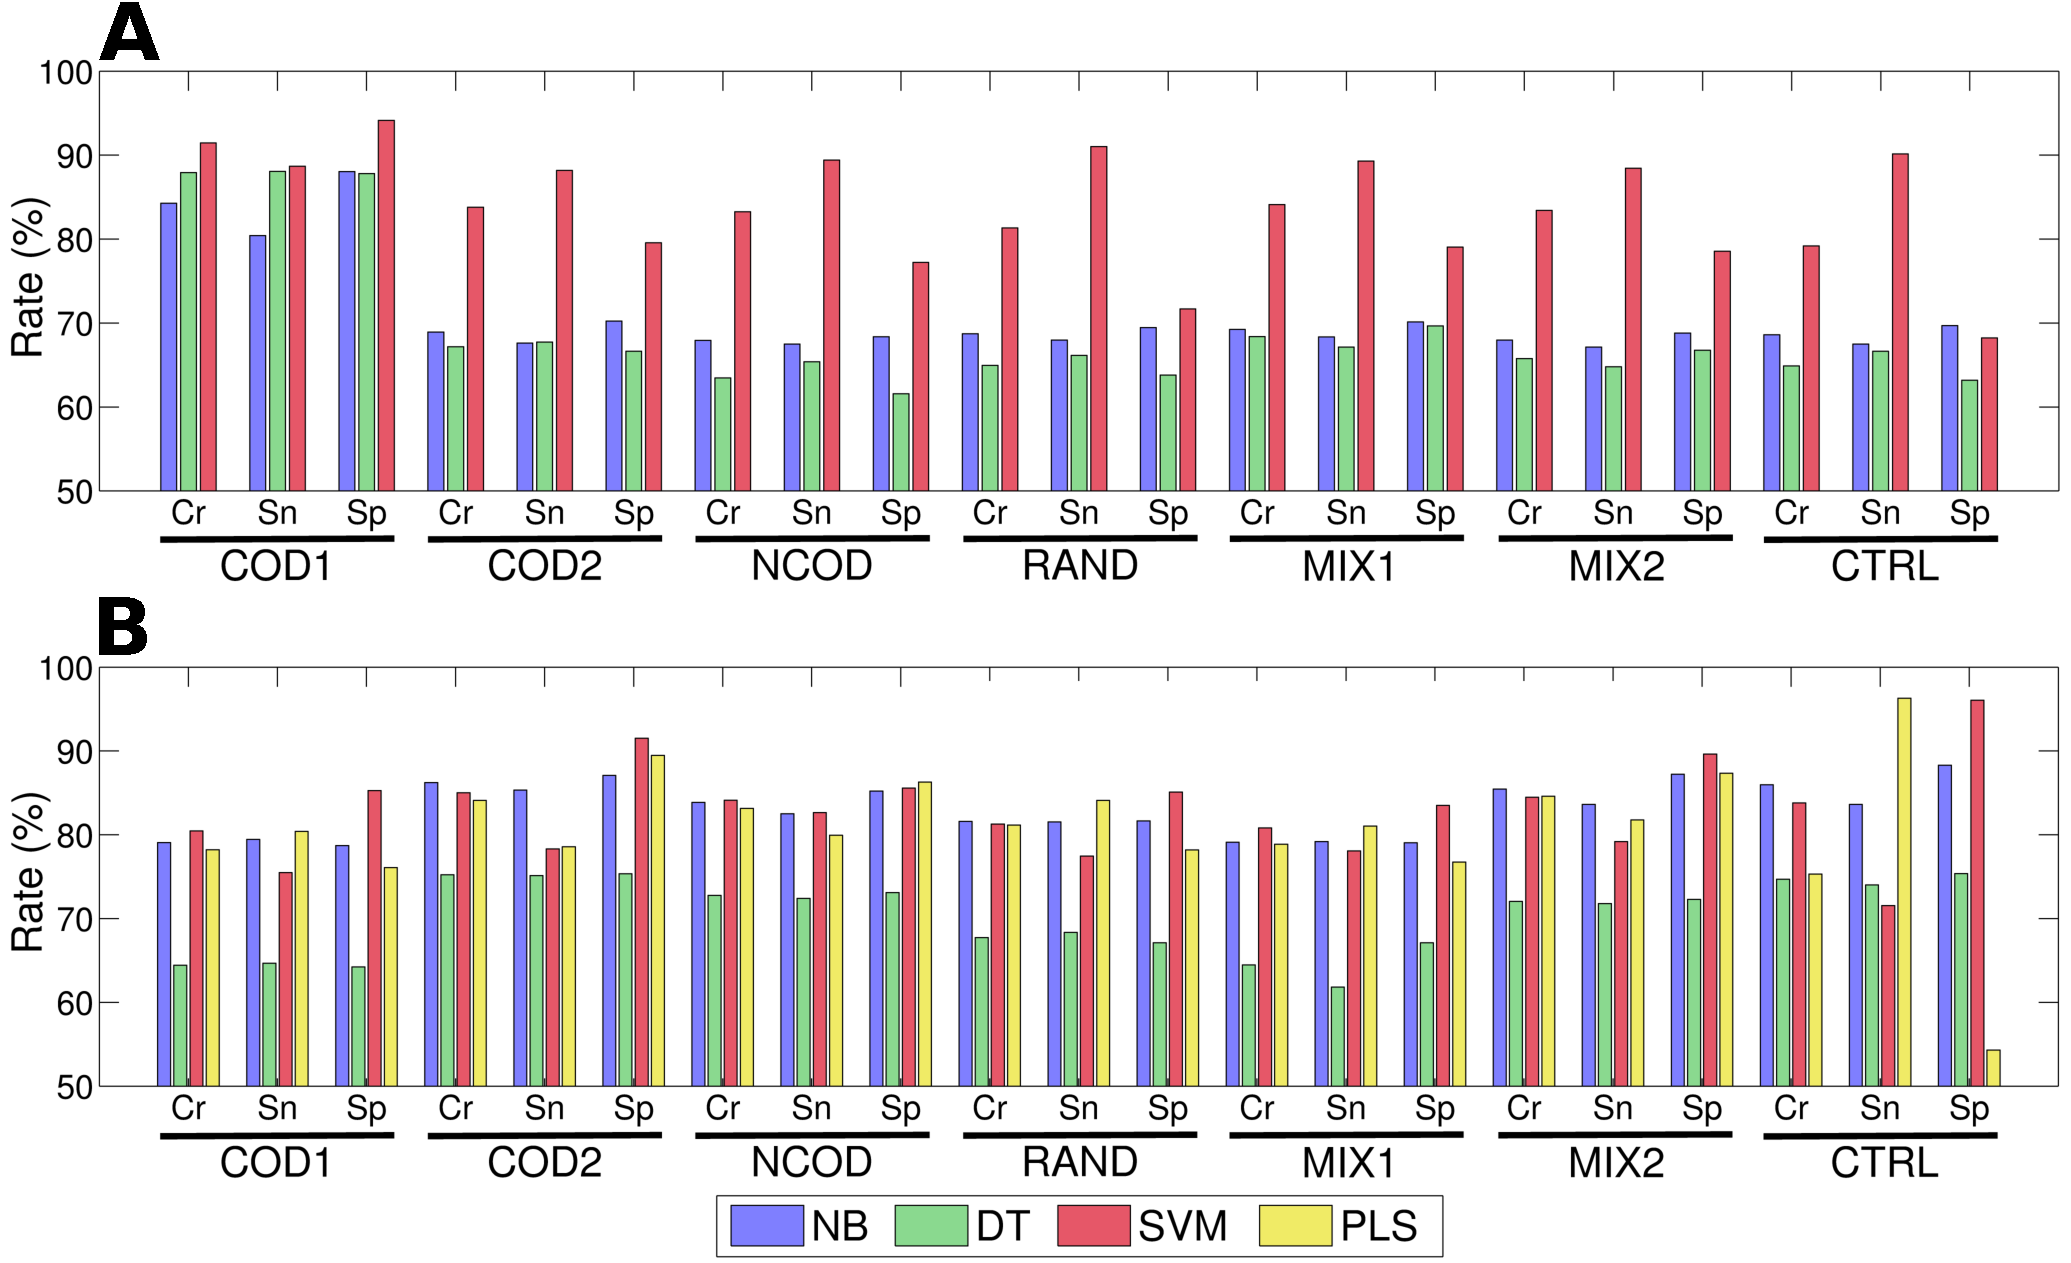
\includegraphics[width=1.0\textwidth]{Figs/Fig.pdf}
    \caption{Correct rate (Cr), sensitivity (Sn) and specificity (Sp) for all classifiers obtained by performing the usual 10-fold cross validation procedure according to case study 1 on the primary sequence datasets ({\bf A}) and features extracted with vw Z-curve ({\bf B}). }
    \label{fig:barplot}
\end{figure*}

The most noticeable result is the significant (p-value regarding specificity $< 10^{-5} $) large values for the statistics obtained by training and testing with {\tt COD1}. This can be explained by the fact that {\tt COD1} was created by extracting sequences from the start of gene ORFs. That is, such a negative example dataset is the only one that has a highly conserved ATG motif (MEME E-value = $1.3\times10^{-8}$). It is important to notice that, although the ATG motif is present in the top-scored MEME result for the {\tt POS} dataset, its position varies within the sequence, differently from {\tt COD1}, which explains the large MEME E-value of $1.3\times10^{19}$. In this categorical scenario, this explains the highly optimistic results for {\tt COD1}, since no other dataset contained an ATG motif among the top 5 enriched motifs based on MEME E-values (see Figure~\ref{fig:meme}).

Now, we turn our analysis to the same data, but, instead of using directly the primary sequences, we consider as attributes the features extracted via the vw Z-curve (Figure~\ref{fig:barplot}B). NB, SVM and PLS performed statistically similarly for all the datasets (p-value $> 0.1$). On the other side, DT had much lower rates in comparison to the other methods (p-values ranging from $4.4\times10^{-4}$ to $5.7\times10^{-8}$). As DT is not very appropriate to deal with numeric attributes, this is an expected result. 

Comparing the results in Figure~\ref{fig:barplot}A and B, one can observe slightly lower (p-value regarding specificity $< 10^{-3} $) results for {\tt COD1} (and {\tt MIX1}, which consists of 50\% of {\tt COD1}). The explanation for this phenomenon probably also lies in the enriched ATG motif present in {\tt COD1}. Since the vw Z-curve captures features in the DNA sequences, the positional information of this ATG motif is diluted in a numerical representation of such triplet. Since both {\tt POS} and {\tt COD1} contain ATG motifs, the classifiers have more difficulty in separating these datasets with similar features. This result supports our idea that the {\tt COD1} dataset provides biased results.

Besides the above statement, no great variations can be observed. Methods based on the use of different features (properties) extracted from the primary sequence as attributes, instead of using directly the sequence, have been gaining popularity. These results also suggest that, in addition to improving prediction power by providing a wider range of information, this methodology minimizes the  biases originating from sequence alignment issues. \\

\begin{table*}
\caption{Specificity for training and testing with SVM classifier -- case study 2}
\begin{center}
    \renewcommand{\arraystretch}{1.2}
    \begin{tabular}{|>{\centering\arraybackslash} m{0.5cm} 
                    |>{\centering\arraybackslash} m{0.5cm} 
                    |>{\centering\arraybackslash} m{1.2cm} 
                    |>{\centering\arraybackslash} m{1.2cm} 
                     >{\centering\arraybackslash} m{1.2cm} 
                     >{\centering\arraybackslash} m{1.2cm} 
                     >{\centering\arraybackslash} m{1.2cm} 
                     >{\centering\arraybackslash} m{1.2cm} 
                     >{\centering\arraybackslash} m{1.2cm} 
                     >{\centering\arraybackslash} m{1.2cm}|}
        \cline{4-10}
            \multicolumn{1}{c}{} & \multicolumn{1}{c}{} & \multicolumn{1}{c|}{} & \multicolumn{7}{c|}{\centering Testing } \\
        \cline{4-10}
            \multicolumn{1}{c}{} & \multicolumn{1}{c}{} & \multicolumn{1}{c|}{} & COD1 & COD2 & NCOD & RAND & MIX1 & MIX2 & CTRL \\
        \hline
            \multirow{14}{*}{\begin{sideways}Training\end{sideways}} & \multirow{7}{*}{\begin{sideways}Sequence\end{sideways}} & COD1 &
            94.14 & 39.43 & 38.30 & 35.83 & 68.80 & 41.93 & 31.26 \\
            &  & COD2 &
            52.79 & 79.55 & 78.08 & 75.11 & 64.07 & 87.39 & 69.93 \\
            &  & NCOD &
            50.36 & 77.98 & 77.21 & 72.87 & 73.33 & 87.87 & 68.81 \\
            &  & RAND &
            47.98 & 75.73 & 73.67 & 71.67 & 58.39 & 74.80 & 66.06 \\
            &  & MIX1 &
            95.25 & 67.61 & 82.39 & 63.88 & 79.04 & 75.76 & 58.40 \\
            &  & MIX2 &
            54.90 & 87.79 & 87.83 & 73.88 & 70.40 & 78.55 & 69.47 \\
            &  & CTRL &
            48.22 & 73.74 & 74.76 & 71.93 & 59.75 & 74.27 & 68.23 \\
        \cline{2-10}
            & \multirow{7}{*}{\begin{sideways}vw Z-curve\end{sideways}} & COD1 &
            85.29 & 91.91 & 84.88 & 82.14 & 91.84 & 88.29 & 72.98 \\
            &  & COD2 &
            71.44 & 91.51 & 85.16 & 80.11 & 77.84 & 92.66 & 62.13 \\
            &  & NCOD &
            61.69 & 84.84 & 85.58 & 80.50 & 79.72 & 92.08 & 56.43 \\
            &  & RAND &
            69.00 & 87.39 & 89.25 & 85.10 & 78.84 & 88.81 & 69.77 \\
            &  & MIX1 &
            87.33 & 91.06 & 93.60 & 84.96 & 83.49 & 91.96 & 68.15 \\
            &  & MIX2 &
            68.76 & 94.00 & 91.85 & 80.25 & 79.57 & 89.64 & 64.84 \\
            &  & CTRL &
            63.18 & 75.73 & 79.52 & 79.27 & 70.17 & 76.12 & 96.06 \\    
        \hline
    \end{tabular}
\end{center}
\label{table:spe}
\end{table*}

\noindent
{\bf Case study 2}: the performance assessment with different negative datasets \\

In this scenario, we compare the performance of the classifiers when the datasets used for training and testing differ. This case study reflects, for instance, exploratory analyses in which not much information is known for a particular organism and researchers usually apply classifiers built with a particular negative dataset in a genome-wide fashion. Since this comparison generates many performance measurements, we will focus our attention to the SVM classifier, which was shown to provide the best performance in our first case study. Table~\ref{table:spe} provides specificity rates obtained by the application of SVM classifier to all combinations of training and testing sets. The upper part of the table regards the primary sequences datasets, whereas the lower part contains the results for vw Z-curve datasets. 

For primary sequence datasets, the bias generated by the presence of ATG motif in {\tt COD1} is now evident: the specificity rates suffer a dramatic drop when {\tt COD1} is used as a training set and other datasets are used as testing set (first row of the upper part of the table). An interesting result is the fact that, for certain contexts, we can observe higher rates for testing with other dataset rather than the one used to build the classifier. For example, in the case of {\tt MIX2}, the classifiers presented better performance when tested either with {\tt COD2} and {\tt NCOD}. Since the application of novel methodologies will be done in a much noisier environment that the controlled 10-fold cross-validation, this could be seen as an evidence that using multiple datasets is essential for any study.

In addition to the training bias, the use of {\tt COD1} also makes clear a testing bias that can be seen by verifying the low specificity rates when training with other datasets and testing with {\tt COD1} (first column of the upper part of the table). At this context, mixing datasets methodology has proven to minimize this kind of bias, though it is still noticeable its preference for its own instances when testing.

\begin{figure}
\vspace{0.0cm}
    \centering
    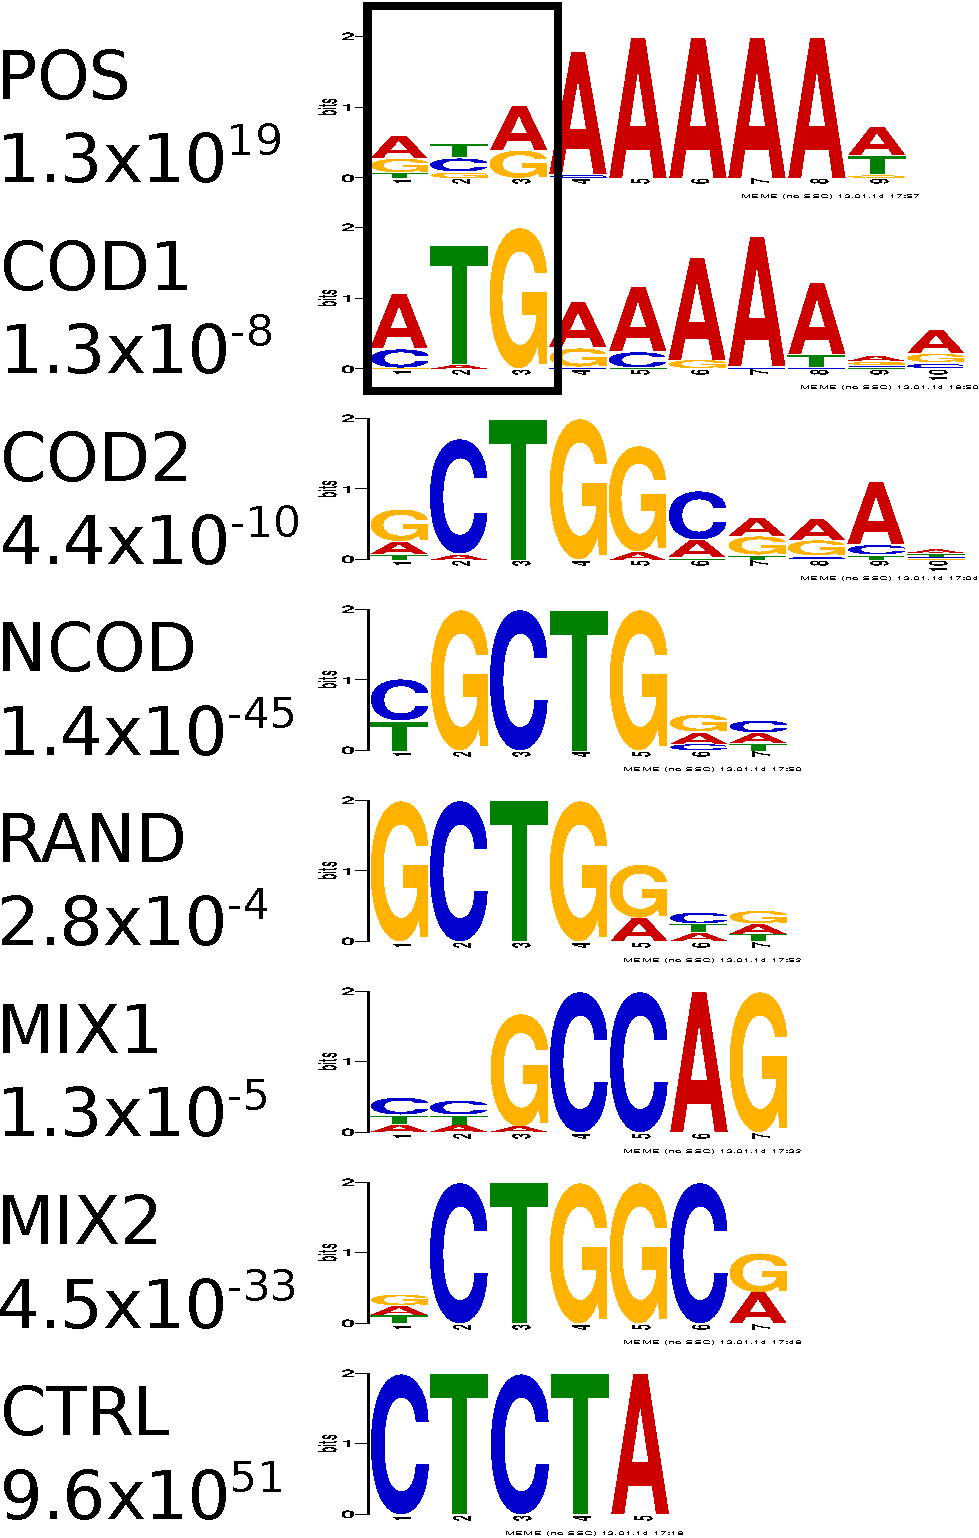
\includegraphics[width=0.425\textwidth]{Figs/MEME.pdf}
    \caption{Top enriched motifs for all datasets studied according to MEME algorithm. Below each dataset name it can be seen the MEME E-value score and, on the right, that dataset's top enriched motif logo. The enriched ATG motifs for the {\tt POS} and {\tt COD1} datasets are marked with a black square.}
    \label{fig:meme}
\end{figure}

In contrast to what we have discussed previously for primary sequence datasets, the results of the vw Z-curve datasets did not present the training bias generated by the conserved ATG in {\tt COD1}. Indeed, the behavior observed was the opposite. When training with {\tt COD1}, the values for testing with {\tt COD2}, {\tt MIX1} and {\tt MIX2} were moderately larger. This unexpected fact led us to conduct a more careful analysis of the structure of these datasets.

In order to do so, we calculated the centroid (average vector) for each dataset in Table~\ref{table:data}. Then, we computed the Euclidean distance between the centroids of each dataset -- inter-dataset distance (see Table~\ref{table:centroid}). Based on this, a probable explanation for the ``inverse'' {\tt COD1} bias for vw Z-curve datasets is that the distance between the centroids of {\tt POS} and {\tt COD2}  is greater than that of between {\tt POS} and {\tt COD1} (respectively, 2.77 and 2.13), while the distance between {\tt COD1} and {\tt COD2 } is much lower (1.62). From a geometrical point of view,  whatever the decision boundary between {\tt POS} and {\tt COD1} is, this same boundary would be able to correctly classify examples from {\tt COD2}, which are closer to the instance in {\tt COD1}, but more distant from the examples in {\tt POS}. \\

\begin{table}[h]
\caption{Distance between the centroids of vw Z-curve datasets}
\begin{center}
    \renewcommand{\arraystretch}{1.2}
    \begin{tabular}{|>{\centering\arraybackslash} m{0.8cm} 
                    |>{\centering\arraybackslash} m{0.6cm} 
                     >{\centering\arraybackslash} m{0.6cm} 
                     >{\centering\arraybackslash} m{0.6cm} 
                     >{\centering\arraybackslash} m{0.6cm} 
                     >{\centering\arraybackslash} m{0.6cm} 
                     >{\centering\arraybackslash} m{0.6cm}
                     >{\centering\arraybackslash} m{0.6cm}|}
        \cline{2-8}
            \multicolumn{1}{c|}{} & POS & COD1 & COD2 & NCOD & RAND & MIX1 & MIX2 \\
        \hline
            COD1 & 2.13 &      &      &      &      &      &      \\
            COD2 & 2.77 & 1.62 &      &      &      &      &      \\
            NCOD & 2.67 & 1.78 & 1.42 &      &      &      &      \\
            RAND & 2.48 & 1.71 & 1.55 & 1.17 &      &      &      \\
            MIX1 & 2.26 & 1.00 & 1.36 & 1.09 & 1.31 &      &      \\
            MIX2 & 2.67 & 1.65 & 0.89 & 0.93 & 1.30 & 1.16 &      \\
            CTRL & 2.55 & 2.43 & 2.75 & 2.56 & 2.38 & 2.42 & 2.59 \\
        \hline
    \end{tabular}
\end{center}
\label{table:centroid}
\end{table}

\noindent
{\bf Discussion} \\

Having analyzed the results of our experiments, we point out to the fact that when applying any methodology in real biological datasets, the learners face data that do not behave so well as in \emph{in silico} experimental pipelines. ``Real world" data consists of general and specific biases and noises that may differ depending on simple actions such as parameter setting. In addition, there are several  types of methodological details that, when incorrectly treated, often lead to biased results. For instance, the dataset {\tt COD1}, used in~\cite{gordon2003,song2011a}, contains a conserved motif. Such a motif, in terms of methods that use primary sequence as input, leads the classifiers generated to classify incorrectly negative examples coming from different distributions.

Moreover, since the goal of any genome-wide prediction technique is to run a classifier and retrieving the regions that are more likely to be enriched for what  is expected it to be, using coding and non-coding negative samples in separate does not necessarily addresses the actual problem. In this context, although our analysis has shown no significant bias related to the {\tt RAND} dataset, the original definition made in~\cite{bland2010} excluded, from the negative dataset, regions within 50bp from the TSS. These regions are known to have lower stress-induced duplex destabilization (SIDD) profile levels, which is a characteristic of a promoter region. Thus, in generating their negative examples in this way, they somehow prevent getting into the dataset segments of genomes that could make the classification, in this context of SIDD profile features, harder. In fact, as demonstrated  in our experiments, when considered out of the SIDD profile context, picking sequences at random from the genome could lead to a dataset that provides a pessimistic view of the classifiers generated.

In summary, we suggest that in studies that the negative examples are hard to determine or supporting evidence is not present, the performance assessment should be accomplished by spanning the largest possible number of scenarios. This includes (1) training and testing with different datasets corresponding to different interpretations of negative samples, (2) generating other datasets, such as combinations of the original datasets, (3) assessing the performance through a wider range of statistics, and (4) exploring other methodological possibilities such as semi-supervised learning and positive only prediction.

\section{Final Remarks}
\label{sec:final}

In this work, we discussed a number of different biases and misinterpretations that often occur in bioinformatics studies concerning the use of supervised learners when negative instances are hard to obtain or define. More specifically, we present an empirical study of the effect of this kind of problem for promoter prediction in {\it E. coli}. To support our discussion we created two evaluation scenarios where a 10-fold cross-validation was applied to 14 different datasets, composed of sequences and features extracted from these sequences, using four machine learning methods. We showed specific and general biases that happened under these circumstances and suggested evaluation criteria to assess the actual performance of novel algorithms over a wide range of bioinformatics fields.

This study can be further expanded to encompass other evaluation scenarios. For example, other features extracted from the sequences can be used such as SIDD profile~\cite{bland2010} or DNA stability based on free energy~\cite{avila2011}. Moreover, the extension of the analyses made in this study to other organisms would probably generate further insights. In this case, more complex negative datasets could be explored such as the ones generated by higher-order Markov chains in order to model nucleotide dependencies. Other possibility is the use of a wider number of classifiers, allowing for a detailed discussion on the specific bias of each learner. One can also compare other approaches, such as non-supervised, semi-supervised or positive sample only learning, to the classical supervised methodology~\cite{cerulo2010,wang2006,yousef2008}.

\section*{Acknowledgment}
We would like to thank K. Song for providing the code regarding the vw Z-curve method.

\def\V{\rm vol.~}
\def\N{no.~}
\def\pp{pp.~}
\def\Pot{\it Proc. }
\def\IJCNN{\it International Joint Conference on Neural Networks\rm }
\def\ACC{\it American Control Conference\rm }
\def\SMC{\it IEEE Trans. Systems\rm , \it Man\rm , and \it Cybernetics\rm }
\def\handb{ \it Handbook of Intelligent Control: Neural\rm , \it
    Fuzzy\rm , \it and Adaptive Approaches \rm }

\bibliographystyle{IEEEtran}
\bibliography{References}

\end{document}
